\documentclass{beamer}
\usetheme{Madrid}
\usepackage[T1]{fontenc}
\usepackage{mathpazo}
\usepackage{graphicx}
\usepackage{booktabs}
\usepackage{tikz}
\usetikzlibrary{positioning,arrows.meta,shapes.geometric,fit,backgrounds,calc}
\definecolor{cetnavy}{RGB}{10,26,63}
\definecolor{cetlight}{RGB}{225,231,242}
\setbeamercolor{structure}{fg=cetnavy}
\setbeamercolor{frametitle}{bg=cetnavy,fg=white}
\setbeamercolor{title}{bg=cetnavy,fg=white}
\setbeamertemplate{navigation symbols}{}
% =====================================================================
%  EDIT YOUR DETAILS HERE — this ONE file feeds every abstract & deck.
%  (Change a value, recompile; all 36 documents update.)
% =====================================================================
\newcommand{\seminarName}{Aflah Muhammed P}      % <-- your full name (guessed from your email; please verify)
\newcommand{\seminarRoll}{TVE00CS000}            % <-- your university register/roll number
\newcommand{\seminarClassRoll}{00}               % <-- your class roll no (the short one)
\newcommand{\seminarGuide}{Prof.\ <Guide Name>}  % <-- your guide
\newcommand{\seminarDept}{Department of Computer Science and Engineering}
\newcommand{\seminarCollege}{College of Engineering Trivandrum}
\newcommand{\seminarShortCollege}{CET}           % shown in the slide footer, e.g. "Aflah Muhammed P (CET)"
\newcommand{\seminarShortTitle}{B.Tech Seminar}  % middle of the slide footer
\newcommand{\seminarDate}{July 31, 2026}
% ---------------------------------------------------------------------
% Optional: put a logo image named  cet_logo.png  in this folder and it
% will appear on every title slide automatically. If absent, it is skipped.
% =====================================================================

\title[\seminarShortTitle]{Search-R1: Reinforcement Learning for Search-Augmented Reasoning}
\author[\seminarName\ (\seminarShortCollege)]{\seminarName \\ \seminarRoll \\ Roll No: \seminarClassRoll \\ Guide: \seminarGuide}
\institute[\seminarShortCollege]{\seminarDept \\ \seminarCollege}
\date{\seminarDate}
\titlegraphic{\IfFileExists{cet_logo.png}{\includegraphics[height=1.1cm]{cet_logo.png}}{}}
\begin{document}
\begin{frame}\titlepage\end{frame}
\begin{frame}{Table of Contents}\tableofcontents\end{frame}
\section{Introduction}
\begin{frame}{Reasoning Meets Search}
\begin{itemize}
\item LLMs reason well but hold static, stale knowledge.
\item Retrieval-augmented generation injects external facts.
\item Complex questions need multi-step, interleaved search.
\item Prompting alone cannot learn a good search policy.
\end{itemize}
\textbf{\textit{Key idea}}
\begin{itemize}
\item Search-R1: use RL to teach \emph{when} and \emph{what} to search.
\item Answers grounded via live search-engine calls.
\end{itemize}
\end{frame}

\section{Literature Survey}
\begin{frame}{Prior Approaches}
\textbf{\textit{Retrieval and prompting}}
\begin{itemize}
\item RAG: retrieve once, then generate.
\item IRCoT: interleave retrieval with chain-of-thought.
\item Search-o1: agentic search via prompting only.
\end{itemize}
\textbf{\textit{RL for reasoning}}
\begin{itemize}
\item DeepSeek-R1: RL elicits reasoning, no search.
\item Supervised tool-use traces: costly and brittle.
\end{itemize}
\end{frame}

\section{Motivation}
\begin{frame}{Why a New Method}
\begin{itemize}
\item Prompt-only search gives no learning signal.
\item Supervised tool traces are hard to annotate.
\item Fixed retrieval ignores the current reasoning state.
\item Model should learn search behavior from outcomes.
\item Multi-hop questions demand several targeted queries.
\end{itemize}
\end{frame}

\section{Problem Statement}
\begin{frame}{The Problem}
\begin{itemize}
\item Train an LLM to interleave reasoning and search.
\item Decide autonomously when and what to query.
\item Keep RL stable with retrieved text in context.
\item Learn without step-level (process) annotations.
\end{itemize}
\end{frame}

\section{Objectives}
\begin{frame}{Goals and Contributions}
\begin{itemize}
\item Unify multi-turn search with RL training.
\item Use only an outcome (correct/incorrect) reward.
\item Stabilize learning via retrieved-token masking.
\item Support both PPO and GRPO; multiple model sizes.
\item Outperform RAG baselines across diverse QA.
\end{itemize}
\end{frame}

\section{Methodology Overview}
\begin{frame}{How Search-R1 Works}
\begin{itemize}
\item Model emits reasoning, then a search query.
\item Engine returns passages as retrieved information.
\item Loop repeats until a final answer is produced.
\end{itemize}
\end{frame}
\begin{frame}{Reason--Search Loop}
\begin{center}
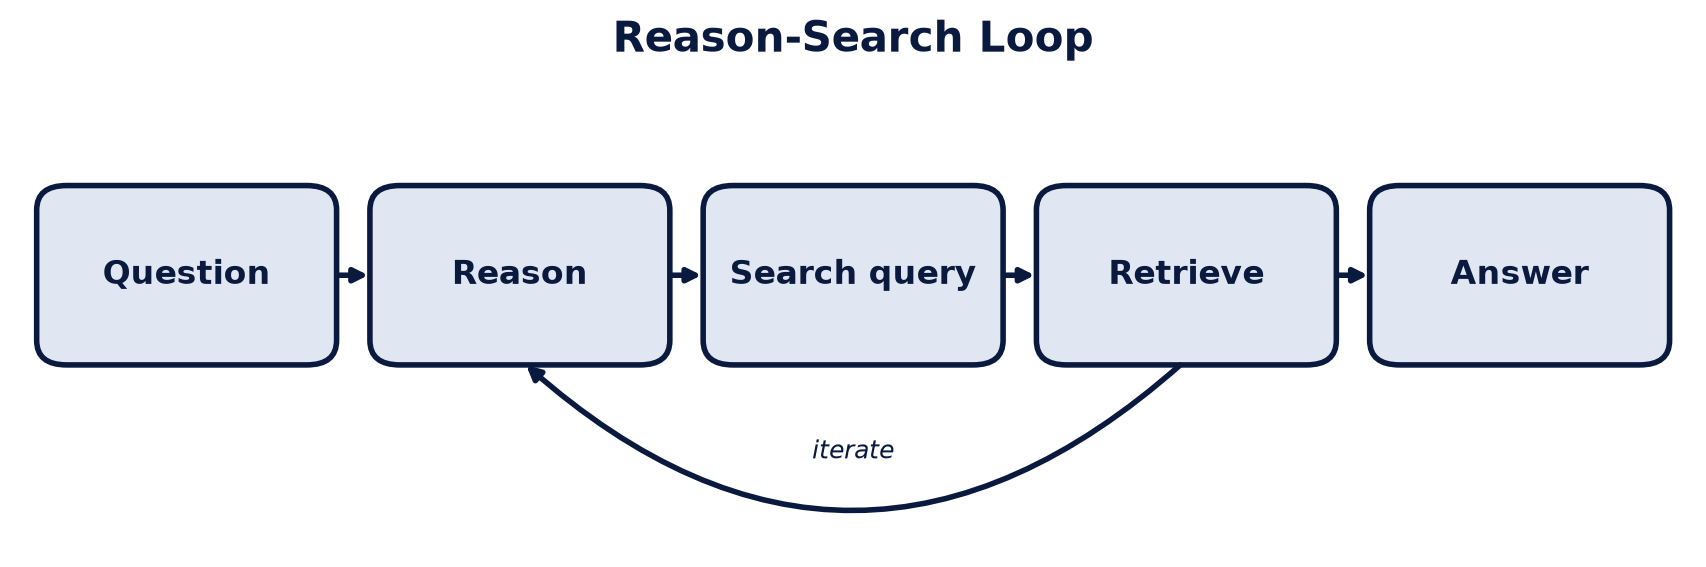
\includegraphics[width=0.9\textwidth,height=0.62\textheight,keepaspectratio]{images/searchr1_1.png}
\end{center}
\end{frame}

\section{System Architecture}
\begin{frame}{Training Stack}
\begin{center}
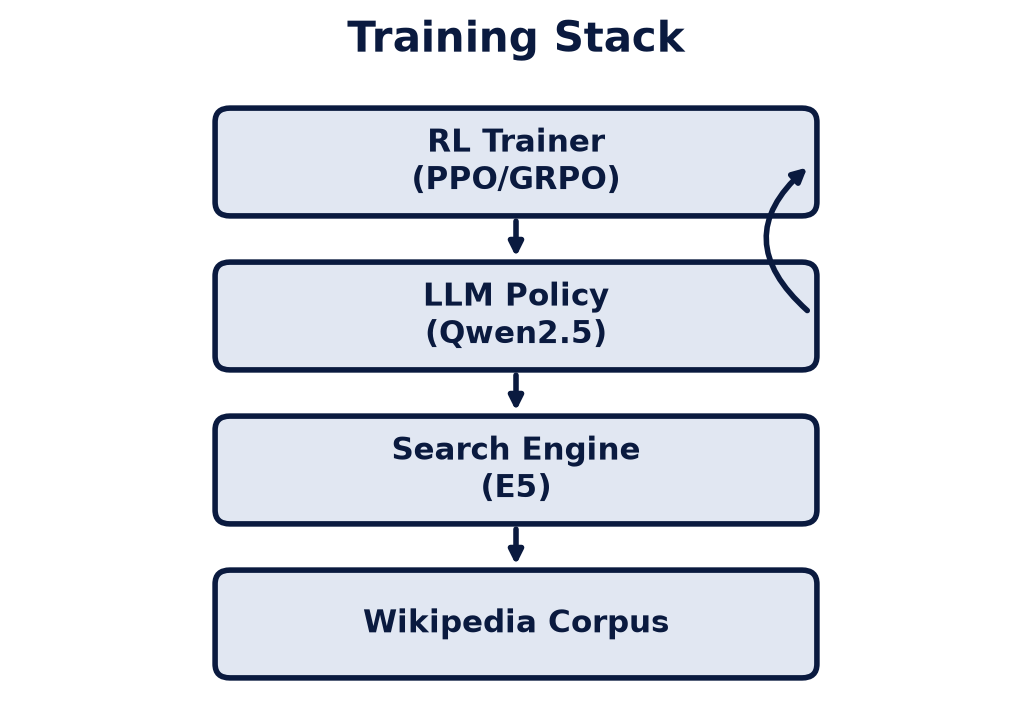
\includegraphics[width=0.9\textwidth,height=0.62\textheight,keepaspectratio]{images/searchr1_2.png}
\end{center}
\begin{itemize}
\item Reward is exact-match; retrieved tokens masked in loss.
\end{itemize}
\end{frame}

\section{Data Collection}
\begin{frame}{Corpus and Retrieval Setup}
\begin{itemize}
\item Corpus: 2018 Wikipedia dump.
\item Retriever: E5 dense, top-3 passages.
\item Training mixes NQ and HotpotQA data.
\item Same retrieval setting for all baselines.
\end{itemize}
\end{frame}
\begin{frame}{Seven QA Benchmarks}
\textbf{\textit{Single-hop}}
\begin{itemize}
\item NQ, TriviaQA, PopQA.
\end{itemize}
\textbf{\textit{Multi-hop}}
\begin{itemize}
\item HotpotQA, 2WikiMultiHopQA, MuSiQue, Bamboogle.
\end{itemize}
\end{frame}

\section{Model Development}
\begin{frame}{Method and Training Details}
\begin{itemize}
\item Base models: Qwen2.5-3B and 7B (base \& instruct).
\item Rollout uses special tokens: \texttt{think}, \texttt{search}, \texttt{information}, \texttt{answer}.
\item Reward: exact match on the final answer only.
\item Loss masking drops all retrieved (information) tokens.
\item Implemented on the veRL RL framework.
\end{itemize}
\end{frame}

\section{Results}
\begin{frame}{Main Findings}
\begin{itemize}
\item About 41\% relative gain (7B), 20\% (3B) over RAG.
\item Search-R1-7B average EM $\approx$ 0.431 vs RAG $\approx$ 0.304.
\item Gains on both single- and multi-hop QA.
\item PPO more stable; GRPO faster but can collapse.
\end{itemize}
\end{frame}
\begin{frame}{Search-R1 vs RAG (7B)}
\begin{center}
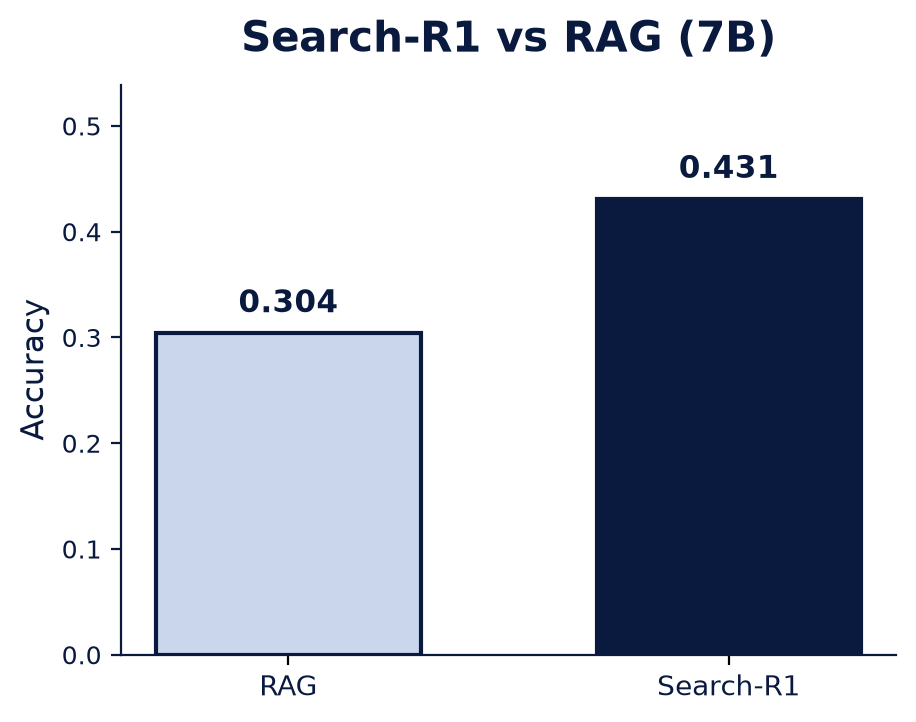
\includegraphics[width=0.9\textwidth,height=0.62\textheight,keepaspectratio]{images/searchr1_3.png}
\end{center}
\begin{itemize}
\item Average exact match, Qwen2.5-7B, seven QA datasets.
\end{itemize}
\end{frame}

\section{Discussions}
\begin{frame}{Why It Works}
\begin{itemize}
\item Model learns to search only when needed.
\item Masking stops it copying retrieved tokens.
\item Outcome-only reward suffices for search behavior.
\item Instruct models converge faster; base models catch up.
\end{itemize}
\end{frame}

\section{Challenges}
\begin{frame}{Limitations}
\begin{itemize}
\item Only outcome reward, no process-level signal.
\item Knowledge limited to the Wikipedia corpus.
\item Bounded interaction and turn budget.
\item RL training cost; sensitive to retrieval quality.
\end{itemize}
\end{frame}

\section{Future Work}
\begin{frame}{Directions Ahead}
\begin{itemize}
\item Richer process- or uncertainty-aware rewards.
\item Dynamic retrieval triggered by model confidence.
\item Diverse tools beyond a text search engine.
\item Multimodal and multi-source reasoning.
\end{itemize}
\end{frame}

\section{Conclusion}
\begin{frame}{Takeaways}
\begin{itemize}
\item RL trains LLMs to search while reasoning.
\item Simple outcome reward plus token masking works.
\item Large, consistent gains over RAG baselines.
\item Framework, models, and code released openly.
\end{itemize}
\end{frame}

\section{References}
\begin{frame}{References}
\footnotesize
\begin{itemize}
\item B. Jin, H. Zeng, Z. Yue, et al., ``Search-R1: Training LLMs to Reason and Leverage Search Engines with Reinforcement Learning,'' arXiv:2503.09516, 2025.
\item DeepSeek-AI, ``DeepSeek-R1: Incentivizing Reasoning Capability in LLMs via Reinforcement Learning,'' arXiv:2501.12948, 2025.
\item X. Li, G. Dong, J. Jin, et al., ``Search-o1: Agentic Search-Enhanced Large Reasoning Models,'' arXiv:2501.05366, 2025.
\end{itemize}
\end{frame}
\begin{frame}\vfill\centering{\Huge Thank You}\vfill\end{frame}
\end{document}
